%%%%%%%%%%%%%%%%%%%%%%%%%% author.tex %%%%%%%%%%%%%%%%%%%%%%%%%
%
% sample root file for your contribution to a "contributed book"
%
% "contributed book"
%
% Use this file as a template for your own input.
%
%%%%%%%%%%%%%%%%%%%%%%%% Springer-Verlag %%%%%%%%%%%%%%%%%%%%%%%%%%

\documentclass{svmult}

\usepackage{amsmath}
\usepackage{amsfonts}
%\usepackage{amssymb}
\usepackage{color}
\usepackage{url}
\usepackage{verbatim}
\usepackage[dvipdfm]{graphicx} % add

%\usepackage{makeidx}         % allows index generation
\usepackage{graphicx}        % standard LaTeX graphics tool
                             % when including figure files
%\makeindex             % used for the subject index
                       % please use the style sprmidx.sty with
                       % your makeindex program

%%%%%%%%%%%%%%%%%%%%%%%%%%%%%%%%%%%%%%%%%%%%%%%%%%%%%%%%%%%%%%%%%%%%%
%\newtheorem{theorem}{Theorem}[section]
%\newtheorem{conjecture}[theorem]{Conjecture}
%\newtheorem{corollary}[theorem]{Corollary}
%\newtheorem{proposition}[theorem]{Proposition}
%\newtheorem{lemma}[theorem]{Lemma}
%\newdef{definition}[theorem]{Definition}
%\newdef{remark}[theorem]{Remark}

% \def\F2{{\mathbb F}_2}
% \def\wt{{\rm wt}}
% \def\wo{{\rm wt}_o}
% \def\wf{{\rm wt}_f}
% \def\UL{{\rm ul}}
% \def\bx{{{\mathbf x}}}
% \def\by{{{\mathbf y}}}
% \def\bz{{{\mathbf z}}}
% \def\bw{{{\mathbf w}}}
% \def\bu{{{\mathbf u}}}
% \def\im{{\mathrm{Im}}}
% \def\ker{{\mathrm{Ker}}}
% \def\id{{\mathrm{Id}}}
% \def\tr{{\mathrm{tr}}}

\def\bbf2{\ifmmode \mathbb{F}_2 \else $\mathbb{F}_2$ \fi}
%\newcommand{\bbf2}{{\ifmmode \mathbb{F}_2 \else $\mathbb{F}_2$ \fi}}

%%%%%%%%%%%%%%%%%%%%%%%%%%%%%%%%%%%%%%%%%%%%%%%%%%%%%%%%%%%%%%%%%%%%%
\begin{document}
%\newcommand{\bbf2}{\ifmmode \mathbb{F}_2 \else $\mathbb{F}_2$ \fi}
\newcommand{\mmod}{\textrm{mod}\,}
%%%%%%%%%%%%%%%%%%%%%%%%%%%%%%%%%%%%%%%%%%%%%%%%%%%%%%%%%%%%%%%%%%%%%

%\title*{Ultra-Fast Low-Discrepancy Points}
%\titlerunning{Fast Points}
%\title*{A uniform real random number generator obeying the IEEE 754
%  format using an affine transition}
\title*{A PRNG specialized in double precision floating point numbers
  using an affine transition}

\titlerunning{A PRNG specialized in double precision floating point numbers}

% \author{
% Usain Bolt\inst{1}\and
% Michael Phelps\inst{2}
% }
\author{Mutsuo Saito\inst{1}\and
Makoto Matsumoto\inst{2}}
% Use \authorrunning{Short Title} for an abbreviated version...
%
% \institute{
% Departement of Superhumans \\
% Lightning Yellow High School\\
% Kingston, Jamaica\\
% \url{http://en.wikipedia.org/wiki/Usain_Bolt}
% \and
% Deep Blue Swimming Pool \\
% University of Baltimore, USA \\
% \url{http://en.wikipedia.org/wiki/Michael_Phelps}
% }
\institute{
Dept.\ of Math.\ Hiroshima University
\texttt{saito@math.sci.hiroshima-u.ac.jp}
\and 
Dept.\ of Math.\ Hiroshima University
\texttt{m-mat@math.sci.hiroshima-u.ac.jp}
}

\maketitle
%%%%%%%%%%%%%%%%%%%%%%%%%%%%%%%%%%%%%%%%%%%%%%%%%%%%%%%%%%%%%%%%%%%%%
            
\begin{abstract} 
  We propose a pseudorandom number generator specialized to
  generate double precision floating point numbers in IEEE 754 format.

  The generator makes pseudorandom 64-bit patterns with the most
  significant 12-bit is specified, so that they represent floating
  point numbers in the range [1,2) obeying the IEEE 754 format in
  memory, using an $\mathbb{F}_2$ affine transition.

  Here, the affine means $x \mapsto Ax+c$ where
  $x$ is a state vector, $A$ is an $\mathbb{F}_2$
  matrix, and $c$ is a constant vector. 
  %This constant
  %is necessary to fix the most significant bits.
  By a slight modification of the classical linear case,
  one can obtain the (lower bound of) period and the dimension of
  equi-distribution of the generator.

  Using SIMD instruction set, we designed dSFMT (double precision floating
  point SFMT), which generates two floating point numbers at one recursion.
  The generation speed is almost same or faster than Mersenne Twister's
  single precision floating point number generation.
\end{abstract}
%%%%%%%%%%%%%%%%%%%%%%%%%%%%%%%%%%%%%%%%%%%%%%%%%%%%%%%%%%%%%%%%%%%%%

\section {Introduction}
\label{sec:intro}

Recently, the scale of simulations is getting larger, and faster
pseudorandom number generators (PRNGs) are required. The power of CPUs
for usual personal computers are now sufficiently strong for such
purposes, and the necessity of efficient PRNGs for CPUs on PCs is
increasing.

We proposed a fast pseudorandom number generator, SIMD-oriented Fast
Mersenne Twister\cite{SFMT} (SFMT) in MCQMC 2006.  SFMT is a successor
of Mersenne Twister\cite{MT} (MT) and faster than the original and has
better equidistribution property.

SFMT is based on a Single Instruction Multiple Data\cite{wiki:SIMD}
(SIMD) feature of recent CPUs. The specialization in hardware made
speed up of SFMT. We also proposed another specialization, block
generation which returns large block of pseudorandom numbers by one
call.  Both of them have been widely known as a technique of speed
up.  Generally saying, specialization is a possible choice to make a
faster PRNG.

We are interested in scientific simulations, and most scientific
Monte-Carlo simulation requires great deal of floating point
pseudorandom numbers.  In this article, we describe about a PRNG
specialized in generating floating point numbers.

%%%%%%%%%%%%%%%%%%%%%%%%%%%%%%%%%%%%%%%%%%%%%%%%%%%%%%%%%%%%%%%%%%%%%
\subsection{Generating floating point numbers}
\label{sec:floating}

Usually, floating point pseudorandom numbers are obtained by
converting integer pseudorandom numbers, because recursion in floating
point numbers accumulates errors, which sometimes have different values
in different CPUs. Generating integer number numbers (which is exact and
fast) and converting it by multiplying a constant is usual way,
however this multiplication has conversion from a integer to
a floating point number, hence the conversion is slow.

An idea to make the conversion fast is using bit operations on integer
number to fit to IEEE 754 floating point format. For example in C
language, to convert 64-bit integer \texttt{x} to double precision floating
point number \texttt{y} is done by:
\begin{verbatim}
   x = (x >> 12) | 0x3FF0000000000000ULL;
   y = *((double *)&x);
\end{verbatim}, more appropriate way in C is to use \textbf{union}.

This method was known at latest in 1997. Anger Fog used this method in
his open source library\cite{web:Fog}.  Others found this method
independently around the year.

Another idea is to convert the unsigned integer to the same bit-sized
signed integer, then (signed) floating point number. The reason why
this method is fast is that implicit conversion uses signed integer
which size is larger than unsigned one. (c.f. \cite{doornik})

Thinking about \bbf2-linear generator like MT, its recursion is done
in \bbf2 vector space and its output vectors are considered as
integers.  In this article, we propose an \bbf2-linear generator whose
output vectors can be regarded as floating point numbers.

%%%%%%%%%%%%%%%%%%%%%%%%%%%%%%%%%%%%%%%%%%%%%%%%%%%%%%%%%%%%%%%%%%%%%
\subsection{IEEE double precision floating point format}
\label{sec:ieee}

IEEE Standard for Binary Floating-Point Arithmetic (ANSI/IEEE Std
754-2008)\cite{ieee754} is the most widely-used standard for
floating-point numbers. The standard was defined in 1985 and revised
in 2008. Here we treat the 64-bit binary format, defined in 1985
standard and also available in 2008 standard.  Figure~\ref{fig:ieee}
shows the 64-bit binary format, which has 1 sign bit, 11 exponent bits
and 52 fraction bits.

\begin{figure}
  \begin{center}
    \includegraphics[width=0.7\linewidth]{ieee.pdf}
    \caption{sign bit, exponent bits and fraction bits of double
      precision floating point number}
    \label{fig:ieee}
  \end{center}
\end{figure}

Table~\ref{tab:ieee} shows how floating point numbers are described in
the format. Most of numbers are normalized. The exponent part $e$ is
adjusted so that the fraction part has a number $f (1 \le f < 2)$, and
$e$ has an offset 1023, then the total of the format shows the number
$f \times 2^{e - 1023}$. And the first 1 of $f$ is omitted in the
format because it is always 1.

\begin{table}[h]
  \begin{center}
    \begin{tabular}{|l|c|c|c|} \hline
      & exponent & fraction & represented number \\ \hline
      zero & 0 & 0 & $\pm 0$ \\ \hline
      denormalized number & 0 & $\neq$ 0 
      & $\pm 0.\texttt{xxxx} \times 2^{-1022}$ \\ 
      \hline
      $\infty$ & 2047 & 0 & $\pm\infty$ \\ \hline
      NaN & 2047 & $\neq$ 0 & Not a Number \\ \hline
      normalized number & 
      other & any & 
      $\pm 1.\texttt{xxxxx} \times 2^{e - 1023}$ \\ \hline
    \end{tabular}
    \caption{Description of double precision floating point
      number. \texttt{xxxx} shows the bit pattern of fraction part.}
    \label{tab:ieee}
  \end{center}
\end{table}
if sign bit is 0 and exponent part (11 bit) is 0x3ff,
then the format represent a normalized number in the range [1, 2).

Because of the format of normalized number, We decided to design a
PRNG whose output is uniformly distributed in the range [1, 2).
\begin{note}
  A normalized number has additional 1 bit and the exponent part is
  adjusted so that the integer part only has this additional 1 bit.
  Therefore this format has 53-bit precision though it has only 52-bit
  fraction part. On the other hand, our generator has 52-bit precision
  because the exponent part is fixed.
\end{note}
%%%%%%%%%%%%%%%%%%%%%%%%%%%%%%%%%%%%%%%%%%%%%%%%%%%%%%%%%%%%%%%%%%%%% 
\section{Theoretical base}
\label{sec:base}

Our new generator is based on Linear Feedback Shift Register (LFSR)
like MT. Moreover it has additional memory called `lung'.  LFSR with
additional memory is called Pulmonary LFSR.

%%%%%%%%%%%%%%%%%%%%
\subsection{LFSR and Pulmonary LFSR}
\label{sec:pulmonary}

We identify the set of bit \{0, 1\} with the two element field \bbf2.
This means that every arithmetic operation is done modulo 2.  A
$\mathbf{b}$-bit register or memory is identified with a horizontal
vector in $\bbf2^b$, and $+$ denotes the sum as vectors (i.e.,
bit-wise exclusive or). We consider an array of $N$ $b$-bit in
computer memory as the vector space $(\bbf2^{b})^N$.

An LFSR method is to generate a sequence $\mathbf{w_0}$,$\mathbf{w_1}$,
$\mathbf{w_2},...$ of elements $\bbf2^b$ by a recursion
\[ \mathbf{w}_{i+N} = g(\mathbf{w}_{i}, ..., \mathbf{w}_{i + N-1}), \]
where $g$ is an $\bbf2$-linear map $(\bbf2^{b})^N \rightarrow
\bbf2^b$.  In the implementation, this recursion is computed by using
an array \texttt{W[0...N-1]} of $N$ word of $b$-bit size, by the
simultaneous substitutions

\begin{multline*}
    \texttt{W[0]} \leftarrow \texttt{W[1]},\ 
    \texttt{W[1]} \leftarrow \texttt{W[2]}, \ldots,
    \texttt{W[N-2]} \leftarrow \texttt{W[N-1]} \\  
    \texttt{[N-1]} \leftarrow
    g(\texttt{W[0]},\ldots,\texttt{W[N-1]}). 
  \end{multline*}

The first $N-1$ substitutions shift the content of the array, hence
the name of LFSR.  Note that in the implementation we may use an
indexing technique to avoid computing these substitutions, see
\cite[P.28 Algorithm A]{knuth:bible}.  Before starting the generation,
we need to set some values to the state array, which is called the
initialization.

Mersenne Twister\cite{MT} (MT) is an example with
\[
g(\mathbf{w}_0,\ldots,\mathbf{w}_{N-1})=(\mathbf{w}_0|\mathbf{w}_1)A + 
\mathbf{w}_M,
\]
where $(\mathbf{w}_0|\mathbf{w}_1)$ denotes the concatenation of the
$32-r$ most significant bits (MSBs) of $\mathbf{w}_0$ and the $r$
least significant bits (LSBs) of $\mathbf{w}_1$, $A$ is a $(32\times
32)$-matrix for which the multiplication $\mathbf{w} A$ is computable
by a few bit-operations, and $M$ is an integer ($1 < M < N$).  Its
period is $2^{32N-r}-1$, chosen to be a Mersenne prime.  To obtain a
better equidistribution property, MT transforms the sequence by a
suitably chosen $(32\times 32)$ matrix $T$, namely, MT outputs
$\mathbf{x}_0 T , \mathbf{x}_1 T, \mathbf{x}_2 T, \ldots$ (called
tempering).

%LFSR has a problem about slow recovery from the status 
%which have many zero bits and little one bits \cite[\S 7]{well}.

A Pulmonary LFSR method is to generate a sequence
$\mathbf{w_0}$,$\mathbf{w_1}$, $\mathbf{w_2},...$ of elements
$\bbf2^b$ by a recursion
\begin{eqnarray}
  \mathbf{w}_i &=& g(\mathbf{w}_{i-N+1}, ..., \mathbf{w}_{i-1},
  \mathbf{u}_{i-1}), \label{eq:recursion} \\
  \mathbf{u}_i &=& h(\mathbf{w}_{i-N+1}, ..., \mathbf{w}_{i-1},
  \mathbf{u}_{i-1}).
\end{eqnarray}
where $g$ and $h$ are $\bbf2$-linear maps $(\bbf2^{b})^N \rightarrow
\bbf2^b$ and $\mathbf{w}_i, \mathbf{u}_i \in \bbf2^b$.  In the
implementation, $\mathbf{u_i}$ is expected to be kept in a register of
CPU.  The idea of Pulmonary LFSR was appeared in the talk of Hiroshi
Haramoto in MCM 2005, and used in WELL PRNG\cite{WELL} in 2006.

In the case of dSFMT, we need an array which have fixed value
\texttt{0x3ff} in MSBs of its elements.  We can exclude these fixed
bits from our state space, but we have to consider the influence of
the fixed bits to the state space. In this case, the state transition
function is changed from $\bbf2$-linear to $\bbf2$-affine.  Here, the
affine means $x \mapsto Ax+c$ where $x$ is a state vector, $A$ is an
$\mathbb{F}_2$ matrix, and $c$ is a constant vector.

%%%%%%%%%%%%%%%%%%%%
\subsection{Computation of the Period}
\label{sec:period}
%To assure the period of PRNG, we used Mersenne Prime\cite{MT}.

A Pulmonary LFSR that obeys the recursion (\ref{eq:recursion}) may be
considered as an automaton, with the state space $S=\bbf2^{b_u + b_w
  \times (N-1)}$ where $b_u$ is size of vector $u$ and $b_w$ is that of
$w$. And the state transition function $f: S \to S$ is given by
\begin{equation*}
  \begin{split}
    (\mathbf{w}_0, &\ldots,\mathbf{w}_{N-2}, \mathbf{u}_0) \\
    &\mapsto 
    (\mathbf{w}_1,\ldots,\mathbf{w}_{N-2},
    g(\mathbf{w}_0,\ldots,\mathbf{w}_{N-2}, \mathbf{u}_0),
    h(\mathbf{w}_0,\ldots,\mathbf{w}_{N-2}, \mathbf{u}_0)).
  \end{split}
\end{equation*}
As a $b_w$-bit vector generator, the output function is 
\[
  o: S \to {\bbf2}^{b_w}; \quad
  (\mathbf{w}_0, \ldots, \mathbf{w}_{N-2}, \mathbf{u}_0) 
  \mapsto \mathbf{w}_0.
\]

Let $\chi_f$ be the characteristic polynomial of $f:S \to S$.  If
$\chi_f$ is primitive, then the period of the state transition takes
the maximal value $2^{\dim(S)}-1$ \cite[\S3.2.2]{knuth:bible}.  To
avoid the the integer factorization of this number, we use the
Mersenne Primes, which are primes $2^p-1$. Here $p$ is called the
Mersenne exponent, which itself is a prime.

MT and WELL\cite{WELL} discard $r$ specific bits from the
array $S$, so that $nw-r$ is a Mersenne exponent. 
Then, the primitivity of $\chi_f$ is easily checked
by the algorithm in \cite[\S3.2.2]{knuth:bible}.

SFMT adopted another method to avoid the integer factorization, the
reducible transition method (RTM), which uses a reducible
characteristic polynomial with a large primitive factor.  This idea
appeared in \cite{FUSHIMI90} \cite{BRENT}\cite{BRENT-PRIM}.

Let $p$ be the Mersenne exponent, and %$N:=\lceil p/b_w \rceil$.
$N$ is length of array in computer memory which just stores $p$-bit
status space.
Then,
we randomly choose parameters for the recursion of LFSR
(\ref{eq:recursion}).  By applying the Berlekamp-Massey Algorithm to
the output sequence, we obtain $\chi_f(t)$.  (Note that a direct
computation of $\det(tI-f)$ is time-consuming because
$\dim(S)$ is large.)

By using a sieve, we remove all factors of small degree from $\chi_f$,
until we know that it has no irreducible factor of degree $p$, or that
it has a (possibly reducible) factor of degree $p$.  In the latter
case, the factor is passed to the primitivity test described in
\cite[\S3.2.2]{knuth:bible}.

Suppose that we found a recursion with an irreducible factor of
desired degree $p$ in $\chi_f(t)$. Then, we have a factorization
\[
\chi_f=\phi_p \phi_r,
\]
where $\phi_p$ is a primitive polynomial of degree $p$
and $\phi_r$ is a polynomial of degree %$r = wN-p$.
$r$ which is remain bit after $N$ element array stores
$p$ bit.
These are coprime, 
since we assume $p>r$.
Let $\ker(g)$ denote the kernel of a linear transformation $g$.
By putting $V_p:=\ker \left(\phi_p(f)\right)$ 
and $V_r:=\ker \left(\phi_r(f)\right)$,
we have a decomposition into $f$-invariant subspaces
\[
S=V_p \oplus V_r \quad (\dim V_p=p, \ \dim V_r=r).
\]
Note that the characteristic polynomial of 
the restriction $f_p$ of $f$ to $V_p$ is $\phi_p(t)$, and
that of the restriction $f_r$ to $V_r$ is $\phi_r(t)$. 
For any state $s \in S$, we denote $s=s_p+s_r$ for the corresponding
decomposition with $s_p \in V_p$ and $s_r \in V_r$.
Then, the $k$-th state $f^k(s)$ is equal to
$f_p^k(s_p) + f_r^k(s_r)$. 

% This implies that the automaton 
% is equivalent to the sum of two automata $f_p:V_p \to V_p$ and
% $f_r: V_r \to V_r$. To combine two linear automata by sum is 
% well-studied as combined Tausworthe generators or combined LFSRs, 
% see \cite{CLT} \cite{COMBTAUS} \cite{COMBLFSR}.
% Their purpose is to obtain a good PRNG from several simple generators,
% which is different from ours.

The period length of the state transition is the least common multiple
of that started from $s_p$ and that started from $s_r$. Hence, 
if $s_p \neq 0$, then the period is a nonzero multiple of $2^p-1$.

To assure that $s_p \neq 0$, we look small subspace of $S$ whose
dimension is greater than that of $V_r$, i.e, one of $w_i$s or $u$.
Let $V_w$ is this subspace, and $V_{wr} = V_w \cap V_r$.  We can get
the basis of $V_{wr}$ by applying $\phi_p(f)$ to randomly selected $s
\in S$, and check in-dependency of the result vector in $V_{wr}$. Then
we can get the basis of orthogonal space $V_{wo}$ of $V_{wr}$ in $V_w$
by linear algebra. We take one of the basis and call it {\em the
  period certification vector} (PCV).

Inner product of PCV and a vector in $V_{wr}$ is always zero,
hence if inner product of the restriction to $V_w$ of initials state $s$
and PCV is not zero, $s$ is not in $V_r$. For period certification of
PRNG, if the inner product is zero, then change 1 bit of a initial state
so that the inner product becomes one.

For our new generator dSFMT, the state transition function is:
\[
  f': S \to S ; \quad s \mapsto f(s) + c,
\]
where $c \in S$ is a constant vector.  Applying above decomposition,
we can get:
\begin{eqnarray*}
  f'(s) &=& f'_p(s) + f'_r(s) \\
  &=&f_p(s) + c_p + f_r(s) + c_r,
\end{eqnarray*}
where $c_p \in V_p$ and $c_r \in V_r$.

To get $c_p$ (or $c_r$), we need a projection function $P_p: S \to
V_p$ (or $V_r$). Using extended Euclidean algorithm, we can
calculate such polynomial $a(t), b(t)$ that:
\[
a(t)\phi_p + b(t)\phi_r = 1.
\]
This means $b(t)\phi_r = 1 (\mmod \phi_p)$ hence we get the projection
$P_p = b(f)\phi_r(f).$

We concern the affine function $f'_p$. If $\exists z\, f_p(z) = z$,
$z$ is called the fix point of affine function. if z exists, 
$(\textrm{Id}_{V_p} - f_p)(z) = c_p$. In this case,
$\phi_p$ is a characteristic polynomial of $f_p$ and is irreducible,
$(1 - t)$ is coprime with $\phi_p$, then we can get $(1 - t)^{-1} \mmod 
\phi_p$ using extended Euclidean algorithm, and we can get fix point
by assigning $f_p$ into $t$ and applying $c_p.$

%  $\phi_p$ is a characteristic
% polynomial of $V_p$ and is irreducible,
% % therefore $f_p$ does not have
% %eigenvalue 1, this means $f'_p$ have fix point.
% therefore we can calculate
% $a(t), b(t) \in \bbf2[t]$ using extended Euclid method such that:
% \[
% a(t)\phi_p(t) + b(t)(t - 1) = 1,
% \]
% then $b(t)$ is $(t - 1)^{-1} \mmod \phi_p(t).$ Now we get
% $(f_p -\textrm{Id}_{V_p})^{-1}$. Let $z := (f_p -\textrm{Id}_{V_p})^{-1}(c_p)$
% then $f_p(z) = z.$ 

When affine function has a fix point $z$, then
\begin{eqnarray*}
  f'_p(z) &=& f_p(z) + c_p = z \\
  c_p &=& z - f_p(z) \\
  f'_p(s) &=& f_p(s) + z - f_p(z) \\
  f'_p(s) - z &=& f_p(s - z).
\end{eqnarray*}
Hence, the affine function can be regarded as a linear function.  Then
the period of affine function is same as the linear function.  To
assure the period, we subtract the fix point from the initial state
$s_0$ first, then check if the result state is not in
$V_r$. 

%%%%%%%%%%%%%%%%%%%%%%%%%%%%%%%%%%%%%%%%%%%%%%%%%%%%%%%%%%%%%%%%%%%%%
\subsection{Computation of the dimension of equidistribution}
\label{sec:DE}
We briefly recall the definition of dimension of 
equidistribution (cf. \cite{CLT}\cite{COMBTAUS}). 
\begin{definition}\label{def:DE}
A periodic sequence with period $P$
\[
\chi:=\mathbf{x}_0, \mathbf{x}_1, \ldots,
 \mathbf{x}_{P-1}, \mathbf{x}_P=\mathbf{x}_0, \ldots
\]
of $v$-bit integers is said to be {\em $k$-dimensionally equidistributed}
if any $kv$-bit pattern occurs equally often as a $k$-tuple
\[
(\mathbf{x}_i, \mathbf{x}_{i+1}, \ldots, \mathbf{x}_{i+k-1})
\]
for a period $i=0,\ldots, P-1$.
We allow an exception for 
the all-zero pattern, which may occur once less often.
(This last loosening of the condition is technically
necessary, because the zero state does not occur
in an $\bbf2$-linear generator). 
The largest value of such $k$ is called the dimension 
of equidistribution (DE).
\end{definition}

We want to generalize this definition slightly.
We define the $k$-window set of the periodic sequence $\chi$
as
\[
W_k(\chi):=
\{(\mathbf{x}_i, \mathbf{x}_{i+1}, \ldots, \mathbf{x}_{i+k-1}) | 
i =0,1,\ldots, P-1\},
\]
which is considered as a {\em multi-set}, namely, 
the multiplicity of each element is considered. 

For a positive integer $m$ and a multi-set $T$,
let us denote by $m \cdot T$ the multi-set 
where the multiplicity of each element in $T$ is
multiplied by $m$. Then, the above definition of
equidistribution is equivalent to 
\[
W_k(\chi)=(m\cdot \bbf2^{vk}) \setminus \{{\mathbf 0}\},
\]
where $m$ is the multiplicity of the occurrences,
and the operator $\setminus$ means that the multiplicity
of ${\mathbf 0}$ is subtracted by one. 

\begin{definition}
In the above setting, if there exist a positive integer $m$ 
and a multi-subset
$D \subset (m\cdot \bbf2^{vk})$
such that
\[
W_k(\chi)=(m\cdot \bbf2^{vk}) \setminus D,
\]
we say that $\chi$ is $k$-dimensionally equidistributed 
with defect ratio $\#(D)/\#(m \cdot \bbf2^{vk})$, 
where the cardinality is counted with multiplicity. 
\end{definition}
Thus, in Definition~\ref{def:DE}, the defect ratio up to $1/(P+1)$
is allowed to claim the dimension of equidistribution.
If $P=2^{p}-1$, then $1/(P+1)=2^{-p}$. 
In the following, the dimension of equidistribution 
allows the defect ratio up to $2^{-p}$. 

For a $b$-bit integer sequence, its {\em dimension of 
equidistribution at $v$-bit accuracy} $k(v)$
is defined as the DE of the $v$-bit sequence, obtained by extracting
the $v$ MSBs from each of the $b$-bit integers.
If the defect ratio is $1/(P+1)$, 
then there is an upper bound 
\[
k(v) \leq \lfloor \log_2 (P+1) / v \rfloor.
\]
The gap between the realized $k(v)$ and the upper bound is
called the dimension defect at $v$ of the sequence,
and denoted by
$$
d(v):=\lfloor \log_2 (P+1) / v \rfloor -k(v).
$$
The summation of all the dimension defects at
$1 \leq v \leq 32$ is called the total dimension defect, 
denoted by $\Delta$.

$k(v)$ of affine state transition function which have fix point is
almost same that of linear transition function, except that the
exceptional tuple which occurs one less offen is not all zero tuple.

There is a difficulty in computing $k(v)$ when 
a 128-bit vector generator is used as a 32-bit 
(or 64-bit) vector generator. This is possible by
using weighted norm and shifted status, (c.f. \cite{SFMT} \cite{thesis:saito}).


% SFMT generates a sequence
% $\mathbf{x}_0, \mathbf{x}_1, \mathbf{x}_2, \ldots$ of 128-bit integers. 
% Then, they are converted to a sequence of 32-bit integers
% $\mathbf{x}_0[0], \mathbf{x}_0[1], \mathbf{x}_0[2], \mathbf{x}_0[3], \mathbf{x}_1[0], \mathbf{x}_1[1],\ldots$,
% where 
% $\mathbf{x}[0]$ is the 32 LSBs of $\mathbf{x}$, 
% $\mathbf{x}[1]$ is the 33rd--64th bits,
% $\mathbf{x}[2]$ is the 65rd--96th bits,
% and $\mathbf{x}[3]$ is the 32 MSBs. 
% %(This is called the 
% %little-endian system, see 
% %\cite{wiki:endian}).
% %for the notion of endianness, 
% %and \S\ref{sec:portability} for
% %an implementation in a big-endian system). 

% Then, we need to modify the model automaton
% as follows.
% The state space is $S':=S \times \{0,1,2,3\}$,
% the state transition function $f':S' \to S'$ is
% $$
% f'(s,i):=
% \left\{
% \begin{array}{cl}
% (s, i+1) & (\mbox{ if $i<3$}), \\
% (f(s), 0) & (\mbox{ if $i=3$}) \\
% \end{array}
% \right.
% $$
% and the output function is 
% $$o': S' \to \bbf2^{32},\  ((\mathbf{w}_0,\ldots,\mathbf{w}_{N-1}),i) \mapsto \mathbf{w}_0[i].$$

% We fix $1\leq v \leq w$, and let $o_k(s,i)$ be the $k$-tuple
% of the $v$ MSBs of the consecutive $k$-outputs from 
% the state $(s,i)$.
% \begin{proposition}
% Assume that $f$ is bijective.
% Let $k'=k'(v)$ denote the maximum $k$ 
% such that 
% \begin{equation}\label{eq:chi-k-i}
% %o_k(-,i): V_p \subset S \to \bbf2^{kv}, \quad s \mapsto o_k(s,i)
% o_k(-,i): V_p \to \bbf2^{kv}, \quad s \mapsto o_k(s,i)
% \end{equation}
% are surjective for all $i=0,1,2,3$. 
% %Take the initial state $s$ satisfying $s_p \neq 0$.
% Take an initial state $s$ satisfying $s_p \neq 0$.
% Then, the 32-bit output sequence is at least $k'(v)$-dimensionally
% equidistributed with $v$-bit accuracy with defect ratio
% $2^{-p}$.

% Moreover, if $4 < k'(v)+1$, then  
% for any initial state with $s=s_p \neq 0$
% (hence $s_r=0$), the dimension of equidistribution
% with defect ratio $2^{-p}$ is exactly $k'(v)$.
% \end{proposition}
% \begin{proof}
% Take $s \in S$ with $s_p \neq 0$. Then, the 
% orbit of $s$ by $f$ has the form of
% $(V_p - \{0\}) \times U \subset V_p \times V_r$,
% since $p>r$ and $2^p-1$ is a prime.
% %Since the first component of the product has
% %odd order, the orbit of $f'$ has the form of
% %$(V_p - \{0\}) \times U' \times \{0,1,2,3\} \in S$.
% The surjectivity of the linear mapping $o_{k'}(-,i)$
% implies that the image of 
% $$
% o_{k'}(-,i): V_p \times U \to \bbf2^{kv}
% $$
% is $m\cdot \bbf2^{kv}$ as a multi-set for some $m$.
% The defect comes from $0 \in V_p$, whose ratio
% in $V_p$ is $2^{-p}$. Then the first statement follows,
% since $W_{k'}(\chi)$ is the union of the images
% $o_{k'}(-,i)((V_p-\{0\})\times U)$ for $i=0,1,2,3$.

% For the latter half, we define
% $L_i$ as the multiset of the image of 
% $o_{k'+1}(-,i): V_p \to \bbf2^{(k'+1)v}$.
% Because of $s_r=0$, we have $U=\{0\}$, and
% the union of $(L_i-\{0\})$ $(i=0,1,2,3)$ as a multi-set is 
% $W_{k'+1}(\chi)$. If the sequence is $(k'+1)$-dimensionally
% equidistributed, then the multiplicity of
% each element in $W_{k'+1}(\chi)$ is at most
% $2^p\times 4/ 2^{(k'+1)v}$.

% On the other hand, the multiplicity of 
% an element in $L_i$ is equal to 
% the cardinality of the kernel of $o_{k'+1}(-,i)$.
% Let $d_i$ be its dimension. Then by the dimension theorem,
% we have $d_i \geq p-(k'+1)v$, and the equality
% holds if and only if $o_{k'+1}(-,i)$ is 
% surjective.
% Thus, if there is a nonzero element 
% $x \in \cap_{i=0}^3{L_i}$, then its multiplicity
% in $W_{k'+1}(\chi)$ is no less than 
% $4 \times 2^{p-(k'+1)v}$, and since
% one of $o_{k'+1}(-,i)$ is not surjective
% by the definition of $k'$, its multiplicity
% actually exceeds $4 \times 2^{p-(k'+1)v}$,
% which implies that the sequence is not
% $(k'+1)$-dimensionally equidistributed, and
% the proposition follows. Since the codimension 
% of $L_i$ is at most $v$, 
% that of $\cap_{i=0}^3{L_i}$ is at most $4v$.
% The assumed inequality on $k'$ implies the existence
% of nonzero element in the intersection.
% %
% %Since the codimension of 
% %each $L_i$ is at most $v$, the codimension of
% %$\cap_{i=0}^3{L_i}$ is at most $4v$. The inequality
% %in the assumption implies that there are at least 
% %two nonzero vectors $x,y \in \cap_{i=0}^3{L_i}$.
% %Now the inverse image of $x$ by $o_{k'+1}(-,i)$
% %has the same cardinality with its kernel,
% %hence $2^{p-\dim L_i}\geq 2^{p-(k'+1)v}$.
% %
% %If $W_{k'+1}(\chi)$ is $(k'+1)$-dimensionally
% %equidistributed, then the inverse image of
% %
% \end{proof}

% The dimension of equidistribution $k(v)$ depends on 
% the choice of the initial state $s$. The above 
% proposition implies that $k'(v)$ coincides 
% with $k(v)$ for the worst choice of $s$ under the condition 
% $s_p \neq 0$. Thus, we adopt the following definition
% (analogously to $t_l$ in \cite{COMBTAUS}).

\begin{definition}\label{def:virtual}
Let $k$ be the maximum such that
(\ref{eq:chi-k-i}) is satisfied. We call this
the dimension of equidistribution
of $v$-bit accuracy, and denote it simply by $k(v)$.
We have an upper bound $k(v) \leq \lfloor p/v \rfloor$.

We define the dimension defect at $v$
%for SFMT19937 used as 32-bit integer generators
by
$$
d(v):=\lfloor p/v \rfloor - k(v) 
\mbox{ and } \Delta:=\sum_{v=1}^w d(v).
$$
\end{definition}
We may compute $k(v)$ by standard linear algebra.
We used a more efficient algorithm based on 
a weighted norm,
%{\em weighted lattice method} to compute $k'(v)$,
generalizing \cite{CLT}. This will be written 
somewhere else,
because of lack of space.
%rather complicated mathematics, we omit it here
%(we plan another article for this). 

%The algorithm gives a (rather tight) 
%lower bound $k'(v)$ of $k(v)$ for each $v$, 
%and $k'(v) \leq \lceil 19937/v \rceil$ holds
%for SFMT19937.
%Consequently, we redefine the dimension defect for SFMT19937 by
%$$
%d(v):=\lceil 19937/v \rceil - k'(v) 
%\mbox{ and } \Delta:=\sum_{v=1}^w d(v).
%$$
%The meaning of $k'(v)$ and a justification for this 
%definition will be explained in the planned article.


%%%%%%%%%%%%%%%%%%%%%%%%%%%%%%%%%%%%%%%%%%%%%%%%%%%%%%%%%%%%%%%%%%%%%
\section{Implementation}
\label{sec:implement}

The aim of this article is to design and to implement a fast floating
point pseudorandom number generator with sufficient quality suitable
for large scale scientific simulation. We decided to use 128-bit
operation customizable in SIMD feature of modern CPUs because we 
succeeded in SFMT.

We call our new generator dSFMT, which stands for double precision
floating point SIMD-oriented Fast Mersenne Twister. dSFMT is
specialized in generating double precision floating point number in
IEEE 754 format.  We released dSFMT based on this idea in 2007 from
our web page\cite{web:SFMT}.

Here we propose an improved version of dSFMT, dSFMT ver. 2.

%%%%%%%%%%%%%%%%%%%%
\subsection{The recursion of dSFMT}
\label{sec:recursion}

dSFMT ver. 2 is a pulmonary LFSR, whose recursion formulas are:
\begin{eqnarray}
  h(\mathbf{w}_0, ..., \mathbf{w}_{N-2}, \mathbf{u}_0)
  &=& \mathbf{w}_{0}A + \mathbf{w}_{M} + \mathbf{u}_{0}B, \label{eq:dsfmt}
  \\
  g(\mathbf{w}_0, ..., \mathbf{w}_{N-2}, \mathbf{u}_0)
  &=& \mathbf{w}_{0} 
  + h(\mathbf{w}_0, ..., \mathbf{w}_{N-2}, \mathbf{u}_0)C,
\end{eqnarray}
where $\mathbf{w}_0$, $\mathbf{w}_M$, $\mathbf{w}_{N-2}$, and $u$ are
b(= 128) bit element of computer memory, regarding horizontal vectors
in $\bbf2^{128}$, and $A$, $B$, $C$ are sparse $128 \times 128$
matrices over \bbf2 for which $\mathbf{w}A$, $\mathbf{w}B$,
$\mathbf{w}C$ can be computed by a few SIMD operations. These vectors
are kept in an N elements array of computer memory, where
$\mathbf{w}_0$, ..., $\mathbf{w}_{N-2}$ are 0th to (N-2)th element and
$u$ is the last element.

\begin{itemize}
\item 
  $\mathbf{w} A := \mathbf{w} \stackrel{64}{<<} \textrm{SL1}$

  This notation means that $\mathbf{w}$ is regarded as two 
  64-bit memories, and $\mathbf{w} A$ is the result of the left-shift
  of $\mathbf{w}$ by SL1 bits. There is such a SIMD operation in 
  Pentium SSE2, and PowerPC AltiVec SIMD can emulate it.
  SL1 is a parameter $12 \le \textrm{SL1} < 64$.

\item
  $\mathbf{u} B := \mathbf{u}\,\textrm{perm(4, 3, 2, 1)}$

  This notation means that $\mathbf{u}$ is regarded as four
  32-bit memories and $\mathbf{u}\,\textrm{perm(4, 3, 2, 1)}$ is
  the result of reverse the order of 32-bit block in 128-bit.
  The permutation can be done by one SIMD operation.

\item 
  $\mathbf{u} C := (\mathbf{u} \stackrel{64}{>>} 12) 
  + (\mathbf{u}\, \& \,\textrm{MASK})$

  The notation $\mathbf{u} \stackrel{64}{>>} 12$ means that
  $\mathbf{u}$ is regarded as two 64-bit memories like $A$ and
  right-shifted 12 bit.  And the notation $\&$ means 128-bit
  bitwise logical `\textbf{AND}' with a 128-bit constant vector \textbf{MASK}.
  MASK is a concatenation of two 64-bit vectors and each of them has
  12 bits of 0s in their most significant bits.

\end{itemize}
Here is a piece of code to show the recursion written in C language.
\begin{verbatim}
    u[0] = (w0[0] << SL1) ^ wm[0] ^ (u0[1] >> 32) ^ (u0[1] << 32);
    u[1] = (w0[1] << SL1) ^ wm[1] ^ (u0[0] >> 32) ^ (u0[0] << 32);
    w[0] = w0[0] ^ (u[0] >> 12) ^ (u[0] & MASK[0]);
    w[0] = w0[1] ^ (u[1] >> 12) ^ (u[1] & MASK[1]);
\end{verbatim}
where \texttt{\^} and \texttt{\&} means bitwise exclusive `OR' and
`AND' respectively, every array is declared to have two unsigned
64-bit integers and \texttt{w0} is for $w_0$, and so
on. Fig.~\ref{fig:dsfmt} shows the recursion in circuit like diagram.

\begin{figure}
  \begin{center}
    \includegraphics[width=\linewidth]{fig-dsfmt.pdf}
    \caption{Diagram of dSFMT}
    \label{fig:dsfmt}
  \end{center}
\end{figure}

Note that (\ref{eq:dsfmt}) does not have neither constants of affine
transformation, nor \texttt{0x3ff} of IEEE 754 exponent part.  Still,
dSFMT has affine transformation function and generates double
precision floating point number in $[1, 2)$ when initial value $w_0,
..., w_{N-2}$ have \texttt{0x3ff} in their exponet part. This trick
contributed the speed up of dSFMT ver. 2 because extra operations for
setting constants are omitted.

Table~\ref{tab:pcv} shows the sets of fix point and period
certification vector(PCV) corresponds with some Mersenne exponents.

% We checked the following. 
% \begin{proposition}
% The period of SFMT19937 as a 128-bit integer generator is 
% a nonzero multiple of $2^{19937}-1$, if the 32 MSBs of 
% $\mathbf{w}_0$ are set to 
% the value {\tt 6d736d6d} in hexadecimal form.
% \end{proposition}

\begin{table}
  \begin{center}
    \caption{Parameter sets}
    \label{tab:params}
    \begin{tabular}{rrrrrr} \hline
      MEXP & $N$ & $M$ & SL1 & MASK(LOW) & MASK(HIGH) \\ \hline \hline
      521 & 5 & 3 & 25 & \texttt{0x000fbfefff77efff} 
      & \texttt{0x000ffeebfbdfbfdf} \\
      1279 & 13 & 9 & 19 & \texttt{0x000efff7ffddffee} 
      & \texttt{0x000fbffffff77fff} \\
      2203 & 21 & 7 & 19 & \texttt{0x000fdffff5edbfff} 
      & \texttt{0x000f77fffffffbfe} \\
      4253 & 41 & 19 & 19 & \texttt{0x0007b7fffef5feff} 
      & \texttt{0x000ffdffeffefbfc} \\
      11213 & 108 & 37 & 19 & \texttt{0x000ffffffdf7fffd} 
      & \texttt{0x000dfffffff6bfff} \\
      19937 & 192 & 117 & 19 & \texttt{0x000ffafffffffb3f} 
      & \texttt{0x000ffdfffc90fffd} \\ \hline
    \end{tabular}
  \end{center}
\end{table}

% $N$, the size of 128-bit array is 
% $\lceil (\textrm{MEXP} - 128) / 104 \rceil + 1$.
% Parameters $M$, SL1 and mask are randomly selected to fit the
% condition that $0 < M < N - 2$, $ 12 < \textrm{SL1}$ and 
% 12-bit of MSB of mask are all zero and the rest bits has many 1s.
% By trial and error, 
% we searched for a set of parameters of dSFMT,
% with the period being a multiple of Mersenne Prime
% and having good equidistribution properties.
% Taable~\ref{tab:params} shows some parameter sets.

%This value of $\mathbf{w}_0$ assures that $s_p\neq 0$,
%see \cite{PMT} for a way to find such a value.

\begin{table}
  \begin{center}
    \caption{Fix Points and Period certification vectors}
    \label{tab:pcv}
    \begin{tabular}{c|rr} \hline
      MEXP & \multicolumn{1}{c}{Fix Point} 
      & \multicolumn{1}{c}{PCV} \\ \hline \hline
      & \texttt{0xcfb393d661638469} & \texttt{0xccaa588000000000} \\
      521 & \texttt{0xc166867883ae2adb} &\texttt{ 0x0000000000000001} \\ \hline
      & \texttt{0xb66627623d1a31be} & \texttt{0x7049f2da382a6aeb} \\
      1279 & \texttt{0x04b6c51147b6109b} & \texttt{0xde4ca84a40000001} \\ \hline
      & \texttt{0xb14e907a39338485} & \texttt{0x8000000000000000} \\
      2203 & \texttt{0xf98f0735c637ef90} & \texttt{0x0000000000000001} \\ \hline
      & \texttt{0x80901b5fd7a11c65} & \texttt{0x1ad277be12000000} \\
      4253 & \texttt{0x5a63ff0e7cb0ba74} & \texttt{0x0000000000000001} \\ \hline
      & \texttt{0xd0ef7b7c75b06793} & \texttt{0x8234c51207c80000} \\
      11213 & \texttt{0x9c50ff4caae0a641} & \texttt{0x0000000000000001}\\ \hline
      & \texttt{0x90014964b32f4329} & \texttt{0x3d84e1ac0dc82880} \\
      19937 & \texttt{0x3b8d12ac548a7c7a} & \texttt{0x0000000000000001} \\ 
      \hline
    \end{tabular}
  \end{center}
\end{table}

%%%%%%%%%%%%%%%%%%%%%%%%%%%%%%%%%%%%%%%%%%%%%%%%%%%%%%%%%%%%%%%%%%%%%
\subsection{Comparison of speed}\label{sec:comp-speed}
We compared two algorithms: MT19937, SFMT19937, dSFMT ver. 1 19937
and dSFMT ver. 2 19937.
with implementations using and without using SIMD instructions.

We measured the speeds for five different CPUs:
Pentium M 1.4GHz, Pentium IV 3GHz, 
AMD Athlon 64 3800+, and PowerPC G4 1.33GHz.  
In returning the random values, we used two different methods.
One is sequential generation, where one 32-bit random 
integer is returned for one call. 
The other is block generation, where an array
of random integers is generated for one call 
(cf. \cite{knuth:bible}). 
For detail, see \S\ref{sec:block} below. 

We measured the consumed CPU time in second, 
for $10^8$ generations of 32-bit integers. More precisely,
in case of the block generation, we generate $10^5$
of 32-bit random integers by one call, and this is iterated
for $10^3$ times. 
For sequential generation, the same $10^8$
 32-bit integers are generated, one per call.
%To avoid the function call, the code uses 
%an inline declaration. 
We used the inline declaration
{\tt inline} to avoid the function call,
and unsigned 32-bit, 64-bit integer types 
{\tt uint32\_t}, {\tt uint64\_t} defined in 
INTERNATIONAL STANDARD ISO/IEC 9899 : 1999(E) 
Programming Language-C, Second Edition
(which we shall refer to as C99 in the rest of this article).
Implementations without SIMD are written in C99,
whereas those with SIMD use
some standard SIMD extension of C99 supported by 
the compilers icl (Intel C compiler) and gcc.

Table~\ref{tab:speed} summarises the speed comparisons.
 The first four lines list the CPU time
(in seconds) needed to generate $10^8$ 
32-bit integers, for a Pentium-M CPU with the Intel C/C++
compiler. The first line lists the seconds for the
block-generation scheme. The second line shows the 
ratio of CPU time to that of 
SFMT(SIMD). Thus, SFMT coded in SIMD is 2.10 times
faster than MT coded in SIMD, and 3.77 times faster
than MT without SIMD. The third line lists the seconds
for the sequential generation scheme. The fourth line
lists the ratio, with the basis taken
at SFMT(SIMD) block-generation (not sequential). 
Thus, the block-generation of SFMT(SIMD) is 2.00 times
faster than the sequential-generation of SFMT(SIMD).

Roughly speaking, in the block generation, 
SFMT(SIMD) is twice as fast as MT(SIMD),
and four times faster than MT without using SIMD.
Even in the sequential generation case,
SFMT(SIMD) is still considerably faster than MT(SIMD).

\begin{table}[h]
  \begin{center}
    \begin{tabular}{|ll|r|r|r|r|r|} \hline
      && dSFMTv2 & dSFMTv1 & MT & SFMT & SFMT \\
      && (new) & (old) & mask & mask & $\times$ const \\ \hline \hline
      Pentium M & blk & 0.626 & 0.867 & 1.526 & 0.928 & 2.636 \\
      1.4 Ghz & seq & 1.422 & 1.761 & 3.181 & 2.342 & 3.671 \\ \hline
      Pentium 4 & blk & 0.254 & 0.640 & 0.987 & 0.615 & 3.537 \\
      3 Ghz & seq & 0.692 & 1.148 & 3.339 & 3.040 & 3.746 \\ \hline
      core 2 duo & blk & 0.199 & 0.381 & 0.705 & 0.336 & 0.532 \\
      1.83GHz & seq & 0.380 & 0.457 & 1.817 & 1.317 & 2.161 \\\hline
      Athlon 64 & blk & 0.362 & 0.637 & 1.117 & 0.623 & 1.278 \\
      2.4GHz & seq & 0.680 & 0.816 & 1.637 & 0.763 & 1.623 \\ \hline
      PowerPC G4& blk & 0.887 & 1.151 & 2.175 & 1.657 & 8.897 \\
      1.33GHz & seq & 1.212 & 1.401 & 5.624 & 2.994 & 7.712 \\ \hline
    \end{tabular}
    \caption{The CPU time (sec.) for $10^8$ generations of double precision
      floating point numbers,
      for four different CPUs and two different return-value methods. 
      The ratio to the SFMT coded in SIMD is listed, too.}
    \label{tab:speed}
  \end{center}
\end{table}

%%%%%%%%%%%%%%%%%%%%%%%%%%%%%%%%%%%%%%%%%%%%%%%%%%%%%%%%%%%%%%%%%%%%%
\subsection{Dimension of equidistribution}
\label{sec:equidistribution}
We calculated $d(v)$s for our generators, by using method described 
\S~\ref{sec:DE}.

Table~\ref{tab:dd} lists the dimension defects $d(v)$ of dSFMT, for
Mersenne exponent mexp $= 521, 1279, 2203, 4253, 11213, 19937$ and
$v=1,2,\ldots, 52$.  $d(v)$ are small for $1 \le v \le 52$, larger mexp
has larger $d(v)$ for later half of $v$s, still mexp 19937 has total
dimension defect $\Delta$ is $2608$, which is smaller than $4188$ of
SFMT19937 and $6750$ of MT19937.

\begin{table}
  \begin{center}
    \begin{tabular}{|r|rrrrrr||r|rrrrrr|} \hline
      & 521 & 1279 & 2203 & 4253 & 11213 & 19937 
      & & 521 & 1279 & 2203 & 4253 & 11213 & 19937 \\ \hline
      d(1) & 0 & 1 & 0 & 0 & 4 & 0 & d(27) & 0 & 0 & 1 & 1 & 33 & 4 \\
      d(2) & 0 & 1 & 1 & 0 & 0 & 1 & d(28) & 0 & 6 & 7 & 28 & 33 & 10 \\
      d(3) & 0 & 2 & 1 & 0 & 0 & 1 & d(29) & 1 & 5 & 7 & 23 & 28 & 67 \\
      d(4) & 0 & 0 & 0 & 0 & 1 & 1 & d(30) & 3 & 3 & 15 & 18 & 80 & 126 \\
      d(5) & 0 & 0 & 0 & 0 & 0 & 0 & d(31) & 2 & 6 & 13 & 15 & 68 & 107 \\
      d(6) & 0 & 1 & 1 & 0 & 1 & 0 & d(32) & 4 & 4 & 10 & 10 & 58 & 88 \\
      d(7) & 0 & 0 & 0 & 0 & 0 & 1 & d(33) & 6 & 12 & 25 & 43 & 120 & 220 \\
      d(8) & 0 & 0 & 0 & 0 & 0 & 1 & d(34) & 6 & 12 & 23 & 44 & 114 & 202 \\
      d(9) & 0 & 1 & 0 & 0 & 0 & 0 & d(35) & 5 & 11 & 21 & 40 & 105 & 185 \\
      d(10) & 1 & 0 & 0 & 0 & 0 & 0 & d(36) & 5 & 10 & 20 & 37 & 96 & 169 \\
      d(11) & 0 & 0 & 0 & 0 & 0 & 0 & d(37) & 5 & 9 & 18 & 33 & 88 & 155 \\
      d(12) & 0 & 0 & 0 & 0 & 0 & 0 & d(38) & 4 & 8 & 16 & 30 & 80 & 141 \\
      d(13) & 0 & 0 & 0 & 0 & 0 & 0 & d(39) & 4 & 7 & 15 & 28 & 72 & 128 \\
      d(14) & 0 & 0 & 0 & 0 & 0 & 1 & d(40) & 4 & 6 & 14 & 25 & 65 & 115 \\
      d(15) & 0 & 0 & 0 & 0 & 0 & 1 & d(41) & 3 & 6 & 12 & 22 & 58 & 103 \\
      d(16) & 0 & 0 & 0 & 0 & 0 & 1 & d(42) & 3 & 5 & 11 & 20 & 51 & 91 \\
      d(17) & 0 & 0 & 0 & 0 & 0 & 0 & d(43) & 3 & 4 & 10 & 17 & 45 & 80 \\
      d(18) & 0 & 0 & 0 & 0 & 0 & 0 & d(44) & 2 & 4 & 9 & 15 & 39 & 70 \\
      d(19) & 0 & 0 & 0 & 0 & 0 & 0 & d(45) & 2 & 3 & 7 & 13 & 34 & 60 \\
      d(20) & 1 & 0 & 0 & 0 & 0 & 0 & d(46) & 2 & 2 & 6 & 11 & 28 & 50 \\
      d(21) & 0 & 0 & 0 & 0 & 7 & 0 & d(47) & 2 & 2 & 5 & 9 & 23 & 41 \\
      d(22) & 0 & 0 & 0 & 0 & 0 & 134 & d(48) & 1 & 1 & 4 & 7 & 18 & 32 \\
      d(23) & 0 & 0 & 7 & 16 & 22 & 94 & d(49) & 1 & 1 & 3 & 5 & 13 & 23 \\
      d(24) & 0 & 1 & 3 & 9 & 19 & 58 & d(50) & 1 & 0 & 3 & 4 & 9 & 15 \\
      d(25) & 0 & 1 & 0 & 6 & 7 & 25 & d(51) & 1 & 0 & 2 & 2 & 4 & 7 \\
      d(26) & 0 & 0 & 0 & 0 & 0 & 0 & d(52) & 1 & 0 & 1 & 0 & 0 & 0 \\ \hline
      \multicolumn{8}{|l|}{total dimension defect $\Delta$} 
      & 73 & 135 & 291 & 531 & 1423 & 2608 \\ \hline
    \end{tabular}
  \end{center}
  \caption{$d(v)$ of 52-bit fraction part of dSFMTv2.}
  \label{tab:dd}
\end{table}

\begin{remark}
  The number of non-zero terms in $\chi_f(t)$ is an index measuring
  the amount of bit-mixing.  The column \textbf{weight} in
  following table shows the number. These values are almost
  half of the degree of $\chi_f(t)$, which implies good bit-mixing.
\end{remark}

\begin{center}
  The number of non zero term in $\chi_f(t)$
  \begin{tabular}{crrrrrr} \hline
    MEXP & 521 & 1279 & 2203 & 4253 & 11213 & 19937 \\
    weight & 273 & 673 & 1076 & 2233 & 5684 & 9756 \\ \hline
  \end{tabular}
\end{center}
%%%%%%%%%%%%%%%%%%%%%%%%%%%%%%%%%%%%%%%%%%%%%%%%%%%%%%% 
\section{Concluding remarks}
We proposed the double precision floating point SFMT (dSFMT)
pseudorandom number generator, which is a very fast generator with
satisfactorily high-dimensional equidistribution property.

% %\subsection{Trade-off between speed and quality}
% It is difficult to measure the generation speed of a PRNG in a fair way,
% since it depends heavily on the circumstances. 
% The 
% WELL \cite{WELL} generators have the best possible dimensions of 
% equidistribution (i.e. $\Delta=0$)
% for various periods ($2^{1024}-1$ to $2^{19937}-1$).
% %If we use the function call to PRNG
% If we use the function call to the PRNG
% for each generation, then a large part of the CPU time
% is consumed for handling the function call, and in the 
% experiments in \cite{WELL} or \cite{XORSHIFT}, WELL 
% is not much slower than MT. On the other hand, if we avoid
% the function call, WELL is slower than MT for some CPUs, 
% as seen in Table~\ref{tab:speed}. 

% Since $\Delta=0$, WELL has a better quality than MT or SFMT
% in a theoretical sense. 
% However, one may argue whether this difference is 
% observable or not. In the case of an $\bbf2$-linear generator,
% the dimension of equidistribution $k(v)$ of $v$-bit accuracy
% means that
% there is no constant linear relation among the 
% $kv$ bits, but there exists a linear relation among
% the $(k+1)v$ bits, where $kv$ bits 
% ($(k+1)v$ bits) are taken from
% all the consecutive $k$ integers 
% ($k+1$ integers, respectively)
% by extracting the $v$ MSBs from each.
% However, the existence of a linear relation does not necessarily
% mean the existence of some observable bias.
% According to \cite{TESTWEIGHT}, it requires $10^{28}$
% samples to detect an $\bbf2$-linear relation with 
% 15 (or more) terms among 521 bits, by weight distribution test. 
% If the number of 
% bits is increased, 
% the necessary sample size is increased rapidly. Thus, it seems
% that $k(v)$ of SFMT19937 is sufficiently large, far beyond
% the level of the observable bias. 
% On the other hand, the speed of the generator is 
% observable.
% Thus, SFMT focuses more on the speed, for applications
% that require fast generations. 
% (Note: the referee pointed out that statistical
% tests based on the rank of $\bbf2$-matrix is sensitive to 
% the linear relations \cite{TESTU01}, 
% so the above observation is not necessarily true.)

% %\subsection{Trade-off between speed and portability}\label{sec:portability}
% There is a trade-off between the speed and portability.
% %We prepare (1) a standard C code of SFMT, which uses 
% We prepared (1) a standard C code of SFMT, which uses 
% functions specified in C99 only, (2) an optimized C code for
% Intel Pentium SSE2, and 
% (3) an optimized C code for PowerPC AltiVec. The optimized codes require
% %icl (Intel C Compiler) or gcc compiler with suitable options.
% the icl (Intel C Compiler) or gcc compiler with suitable options.
We had put and will keep the newest version of the codes 
in the web page \cite{web:SFMT}.

\section*{Acknowledgements}
This study is partially
supported by JSPS/MEXT Grant-in-Aid for Scientific Research
No.19204002, No.18654021, and JSPS Core-to-Core Program
No.18005.

\bibliographystyle{plain}
\bibliography{sfmt-kanren}
\end{document}
%%%%%%%%%%%%%%%%%%%%%%%%%%%%%%%%%%%%%%%%%%%%%%%%%%%%%%%%%%%%%%%%%%%%%
\section{How to select the recursion and parameters.}
We wrote a code to compute the period and
the dimensions of equidistribution (DE,
see \S\ref{sec:DE}). 
Then, we searched
for a recursion with good DE admitting a fast implementation.  

\section{Recovery from 0-excess states}
%LFSR with a sparse feedback function $g$ has
%the following phenomenon: 
For an LFSR with a sparse feedback function $g$,
we observe the following phenomenon: 
if the bits in the state space 
contain too many 0's and few 1's (called a 0-excess state), then
%this tendency continues for considerable generations,
this tendency continues for many steps,
since only a small part is changed in the state array
%at one generation, and the change is not well-reflected to 
%the next generation because of the sparseness.
at one step, and the change is not well-reflected to 
the next step because of the sparseness.

We measure the recovery time from 0-excess states, 
by the method introduced in \cite{WELL}, as follows.
\begin{enumerate}
\item Choose an initial state with only one bit being 1.
\item Generate $k$ pseudorandom numbers, and discard them.
\item Compute the ratio of 1's among the 
next 32000 bits of outputs
(i.e., in the next 1000 pseudorandom 32-bit integers).
\item Let $\gamma_k$ be the average of the ratio over
all such initial states.
\end{enumerate}
We draw graphs of these ratio $\gamma_k$ $(1 \leq k \leq 20000)$
in Figure~\ref{fig:zero-recovery}
for the following generators: (1) WELL19937c, 
(2) PMT19937 %\cite{PMT},
 (3) SFMT19937, and (4) MT19937. 
%For (1), (2), (3) and (3), the chosen 
%initial states are those with only one bit being 1
%and all the rest 0. For (2*), the 32 MSBs in the first 128-bit
%integer in the state array is fixed to the value 
%{\tt 6d736d6d} in the hexadecimal form, and the initial states
%are those with only one bit being 1, except these 32 bits.
%Setting these 32 bits to this value assures that SFMT19937
%has the period being a nonzero multiple of $2^{19937}-1$,
%see \S\ref{sec:period}.
\begin{figure}
\begin{center}
\vskip -3mm
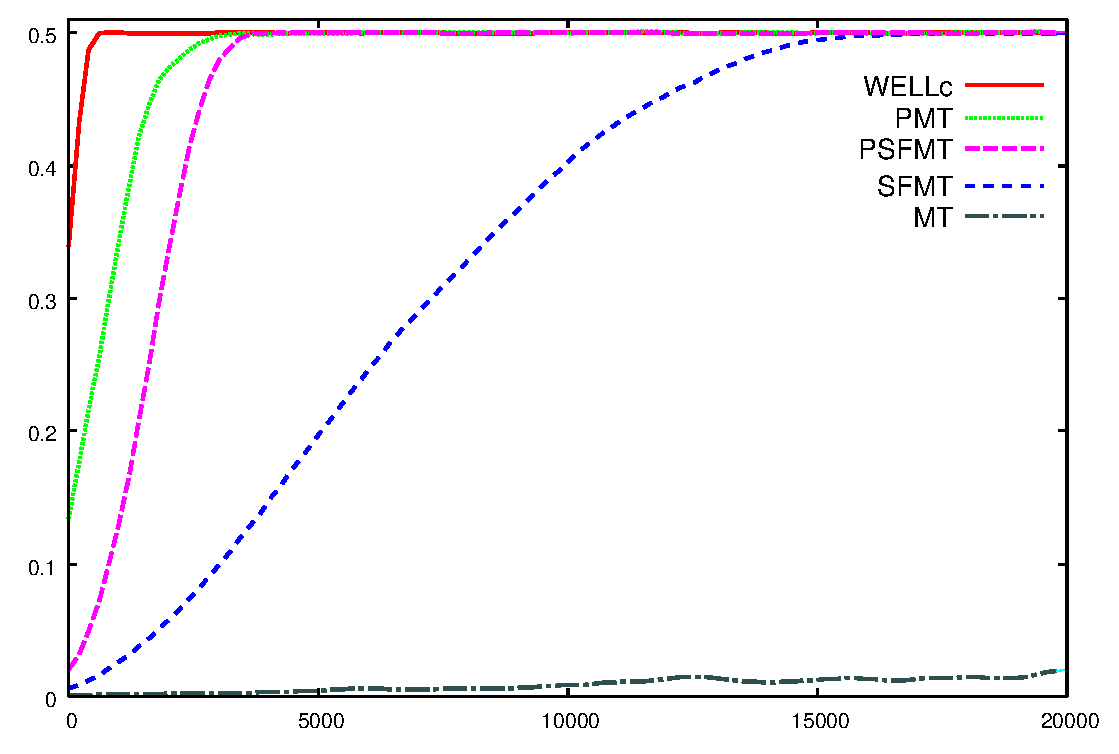
\includegraphics[width=0.7\linewidth]{sfmt-zero.eps}
\end{center}
\caption{$\gamma_k \ (k=0,\ldots,20000)$:
Starting from extreme 0-excess states,
discard the first $k$ outputs and then measure
the ratio $\gamma_k$ of 1's in the next 1000 outputs. 
In the order of the recovery speed: 
(1) WELL19937c, 
(2) PMT19937, (3) SFMT19937, and (3) MT19937.
}\label{fig:zero-recovery}
\end{figure}
Because of its dense feedback, WELL19937c shows
%the fastest recovery among the compared. 
the fastest recovery among the compared generators. 
SFMT is better than MT, since its recursion refers to 
%the previously-computed words (i.e., {\tt W[N-1]} and {\tt W[N-2]}) 
two most recently computed words ({\tt W[N-1]} and {\tt W[N-2]}) 
that acquire new 1s, while
MT refers only to the words generated long before 
({\tt W[M]} and {\tt W[0]}). PMT19937 shows faster recovery 
than SFMT19937, since PMT19937 has two feedback loops.
%(hence the name of Pulmonary Mersenne Twister).
The speed of recovery from 0-excess states 
is a trade-off 
with the speed of generation. 
Such 0-excess states will not happen practically, 
since the probability 
that 19937 random bits have less than $19937\times 0.4$ of 1's 
is about $5.7\times 10^{-177}$.
The only plausible case would be that
a poor initialization scheme gives a 0-excess initial state
(or gives two initial states whose Hamming distance is too small). 
In a typical simulation, the number of 
initializations is far smaller than the number of generations,
therefore we may spend more CPU time in the initialization
than the generation. Under the assumption that
a good initialization scheme is provided, the slower
recovery of SFMT compared to WELL would perhaps not be
a great issue.
% Once we avoid problematic initial states
%by a well-designed initialization, then the recovery 
%speed would not matter.%, in a practical sense. 
%We think the slower recovery of SFMT compared to WELL 
%would not be a great issue, under the assumption that
%a good initialization scheme is provided. 

\end{document}

% LocalWords:  MCQMC denormalized xxxx NaN xxxxx Hiroshi Haramoto MCM nw RTM tI
% LocalWords:  wN th wr wo PCV kv vk sl rrrrrrr MEXP fbfefff efff ffeebfbdfbfdf
% LocalWords:  ffddffee fbffffff fff fdffff edbfff fffffffbfe fffef feff fffd
% LocalWords:  ffdffeffefbfc ffffffdf dfffffff bfff ffafffffffb ffdfffc rr xcfb
% LocalWords:  xccaa xc ae adb xb da aeb xde xf ef fd cb ba xd caae uint IEC le
% LocalWords:  icl dSFMTv const blk Ghz mexp rrrrrr sfmt kanren
